% Toy paper for the AI for Research seminar.
%
% Illustrative only. This skeleton is meant to be filled in by an AI agent
% working from the Stack Overflow Annual Developer Survey data.
% See ../README.md for the workflow.

\documentclass[11pt]{article}

\usepackage[a4paper, margin=2.5cm]{geometry}
\usepackage{graphicx}
\usepackage{booktabs}
\usepackage{hyperref}
\usepackage{natbib}
\usepackage{authblk}

\title{AI-tool adoption and self-reported job satisfaction among professional
software developers: a descriptive analysis of the Stack Overflow Annual
Developer Survey}

\author[1]{Rita Coelho do Vale}
\affil[1]{Universidade Cat\'olica Portuguesa}

\date{\today}

\begin{document}
\maketitle

\begin{abstract}
We use the Stack Overflow Annual Developer Survey \citep{stackoverflow2025survey}
to describe the relationship between professional developers' reported adoption
of AI coding tools and their reported job satisfaction, controlling for years of
professional experience and primary developer role.
We document a small positive cross-sectional association: each step up on a
five-point AI-adoption ordinal is associated with an increase of 0.063 points
on a 0--10 job-satisfaction scale (SE\,=\,0.009; $p < 0.001$; $N = 23{,}722$).
The analysis is purely descriptive.
The survey is observational, selection into the survey is non-random, and both
AI-tool adoption and job satisfaction are self-reported.
We discuss the limits this design imposes on causal interpretation.
This paper is a teaching artefact produced for a seminar on AI for research;
it is not intended for publication.
\end{abstract}

\section{Introduction}

The rapid adoption of AI-assisted coding tools---autocomplete engines,
conversational agents, and code-generation assistants---has made it a
first-order question for researchers, managers, and developers themselves
whether working with such tools is associated with better or worse working
experiences. Surveys of developer populations consistently record rising
AI-tool uptake; what is less clear is whether those who adopt these tools
report different levels of job satisfaction from those who do not.

The present paper takes no stand on causation. We treat the data as a
cross-sectional snapshot and ask only whether there is a descriptive
association between AI-tool adoption and job satisfaction, and whether
that association persists once we account for years of professional
experience and primary developer role. We make no claim that AI tools
improve satisfaction, nor that more satisfied developers are more likely
to adopt AI tools---the data do not allow us to distinguish these
interpretations.

Our contribution is deliberately modest: we provide a transparent, fully
reproducible worked example of how a modest descriptive association can be
documented honestly, with its limits made explicit. This paper is an
artefact produced for a seminar on the use of AI agents in academic
research workflows. The workflow---data download, analysis, figure
generation, and paper compilation---was executed end-to-end with AI
assistance, and the resulting paper is intended to illustrate that
workflow rather than to advance substantive knowledge about AI tools or
job satisfaction.

\section{Data}

We use the Stack Overflow Annual Developer Survey 2025
\citep{stackoverflow2025survey}, an annual self-administered online
survey of software developers worldwide, conducted and released publicly
by Stack Overflow under ODbL\,1.0 and DbCL\,1.0 licences.
The 2025 wave contains 49,191 responses across 172 survey items.

\textit{Analysis sample.} We restrict to professional developers---excluding
respondents whose primary reported role is ``Student'' or whose role falls
into unclassified ``Other'' categories---and drop observations with any missing
value on the four variables used in the analysis (AI-tool use, job
satisfaction, years of professional experience, and developer role).
The resulting analysis sample comprises 23,722 respondents.

\textit{Variables.} \textbf{Job satisfaction} is measured on a continuous
0--10 numeric scale (\texttt{JobSat}), with higher values indicating greater
satisfaction. In the analysis sample the mean is 7.22 (SD\,=\,1.97) and the
median is 8.0. \textbf{AI-tool adoption} is captured by
\texttt{AISelect}, a five-category item asking how frequently the respondent
uses AI tools in their development work. We code this as a zero-to-four ordinal
variable: 0 = ``No, and I don't plan to''; 1 = ``No, but I plan to soon'';
2 = ``Yes, monthly or infrequently''; 3 = ``Yes, weekly''; 4 = ``Yes, daily''.
\textbf{Professional experience} is measured by \texttt{WorkExp}, the number
of years of professional coding experience (mean\,=\,13.6; median\,=\,11.0).
\textbf{Developer role} is the respondent's primary self-reported role,
taken as the first item in \texttt{DevType}; roles with fewer than 500
respondents in the sample are collapsed into ``Other professional''.

\section{Method}

We estimate a linear (OLS) regression of job satisfaction on AI-adoption
ordinal, years of professional experience, and a set of developer-role
fixed effects:
\[
  \texttt{JobSat}_i \;=\;
  \alpha
  \;+\; \beta\,\texttt{AISelect}_i
  \;+\; \gamma\,\texttt{WorkExp}_i
  \;+\; \sum_k \delta_k\,\mathbf{1}[\texttt{role}_i = k]
  \;+\; \varepsilon_i
\]
Standard errors are heteroscedasticity-robust (HC3). The coefficient
$\beta$ is the parameter of primary interest: it captures the average
difference in job satisfaction associated with a one-step increase in
AI-adoption frequency, holding experience and role constant.

We emphasise that this is a cross-sectional regression on observational,
self-reported data. The coefficient $\beta$ is a descriptive partial
correlation, not a causal effect. We run one robustness check: repeating
the main regression on the subsample of respondents with more than five
years of professional experience ($N = 17{,}979$) to assess whether the
association is driven by junior developers.

\section{Results}

Figure~\ref{fig:sat-by-ai} shows mean job satisfaction by AI-adoption category
for all respondents with non-missing values on both variables ($N = 24{,}126$
before additional covariate restrictions).
The pattern is non-monotonic at intermediate adoption levels: ``Monthly''
users report the lowest mean satisfaction (7.11), while ``Daily'' users
report the highest (7.30). Respondents who do not plan to use AI tools
report a mean satisfaction of 7.15. The differences across categories are
statistically distinguishable but substantively small relative to the
within-group standard deviation (approximately 1.9 to 2.0 points).

\begin{figure}[h]
  \centering
  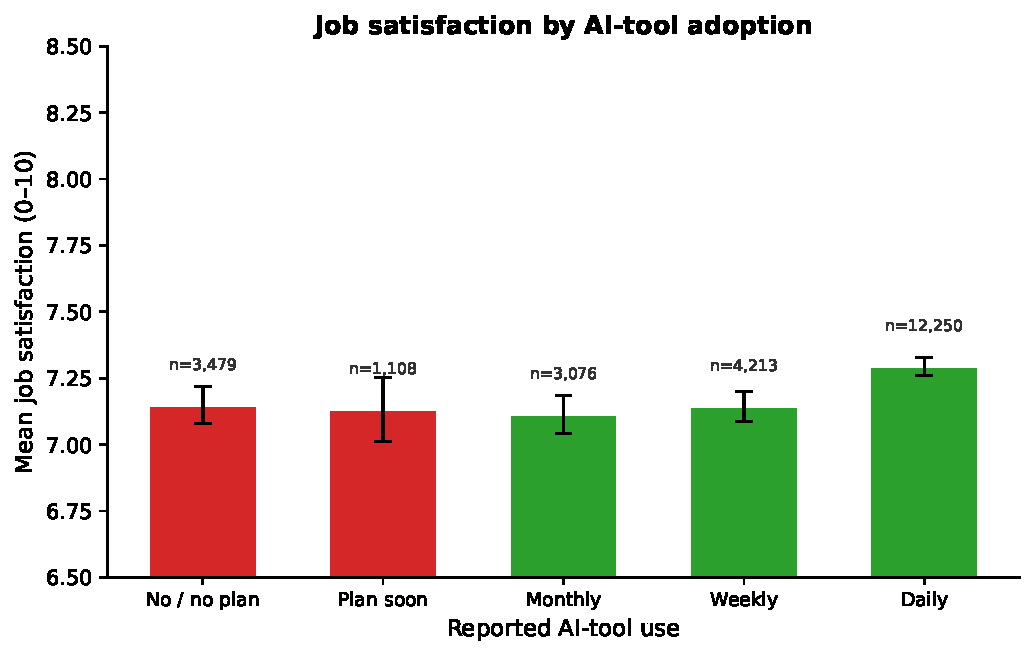
\includegraphics[width=0.85\linewidth]{figures/fig1_satisfaction_by_ai_use.pdf}
  \caption{Mean job satisfaction (0--10 scale, error bars are 95\% confidence
  intervals) by reported AI-tool adoption frequency. ``No / no plan'' and
  ``Plan soon'' respondents report slightly lower mean satisfaction than
  current users, with ``Daily'' users reporting the highest mean (7.30).
  Sample: all respondents with non-missing values on both variables
  ($N = 24{,}126$). Source: Stack Overflow Annual Developer Survey 2025
  \citep{stackoverflow2025survey}.}
  \label{fig:sat-by-ai}
\end{figure}

In the main OLS regression (Table~\ref{tab:reg}), the coefficient on
AI-adoption ordinal is $\hat\beta = 0.063$ (HC3 SE\,=\,0.009;
$p < 0.001$; 95\% CI: [0.044, 0.081]).
This implies that moving from ``No, and I don't plan to'' (0) to ``Yes,
I use AI tools daily'' (4) is associated with a predicted 0.25-point
increase in job satisfaction on the 0--10 scale, holding experience and
role constant. The model explains roughly 1.9\% of the variance in job
satisfaction ($R^2 = 0.019$), indicating that AI-adoption frequency
accounts for a small share of total variation in satisfaction.
In the robustness subsample restricted to respondents with more than five
years of experience, the point estimate is $\hat\beta = 0.079$
(SE\,=\,0.011; $p < 0.001$; $N = 17{,}979$), which does not differ
materially from the full-sample estimate, suggesting the association is
not driven by junior developers.

\begin{table}[h]
\centering
\caption{OLS regression of job satisfaction (0--10) on AI-adoption ordinal.
Heteroscedasticity-robust standard errors (HC3) in parentheses.
$^{*}p<0.05$, $^{**}p<0.01$, $^{***}p<0.001$.}
\label{tab:reg}
\begin{tabular}{lcccc}
\toprule
 & M1 & M2 & M3 (main) & M3 robustness \\
 & Bivariate & + Experience & + Role FE & exp $> 5$ yrs \\
\midrule
AI adoption (0--4) & 0.046$^{***}$ & 0.066$^{***}$ & 0.063$^{***}$ & 0.079$^{***}$ \\
                   & (0.009)       & (0.009)       & (0.009)       & (0.011) \\
Experience (yrs)   &               & 0.023$^{***}$ & 0.021$^{***}$ & 0.019$^{***}$ \\
                   &               & (0.001)       & (0.001)       & (0.002) \\
Role fixed effects & No  & No  & Yes & Yes \\
\midrule
$N$                & 23,722 & 23,722 & 23,722 & 17,979 \\
$R^2$              & 0.001  & 0.015  & 0.019  & 0.018 \\
\bottomrule
\end{tabular}
\end{table}

Figure~\ref{fig:years} shows the distribution of years of professional coding
experience in the analysis sample. The distribution is right-skewed, with a
median of 11 years and a mean of 13.6 years, reflecting the composition of
Stack Overflow's respondent pool toward mid-career and senior developers.

\begin{figure}[h]
  \centering
  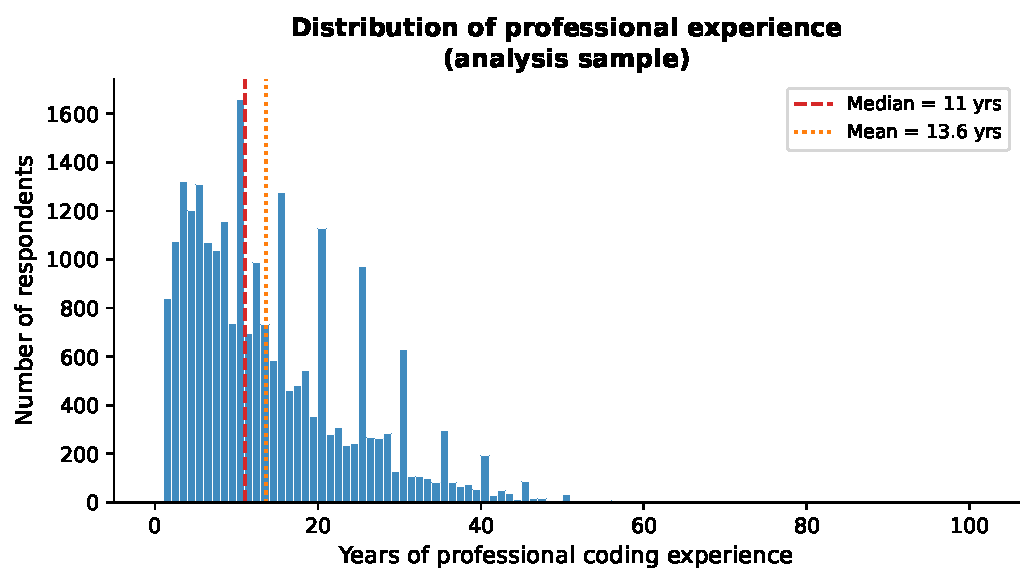
\includegraphics[width=0.85\linewidth]{figures/fig2_years_experience.pdf}
  \caption{Distribution of years of professional coding experience in the
  analysis sample ($N = 23{,}722$). The red dashed line marks the median
  (11 years); the orange dotted line marks the mean (13.6 years). The
  right-skewed distribution indicates that the sample skews toward
  mid-career and senior developers. Source: Stack Overflow Annual Developer
  Survey 2025 \citep{stackoverflow2025survey}.}
  \label{fig:years}
\end{figure}

\section{Limitations}

The following limitations govern any interpretation of these results.
We list them explicitly because, in our view, a transparent account of
what the data cannot show is more valuable for teaching purposes than
a confident-sounding but under-qualified conclusion.

\textbf{Non-random selection into the survey.}
The Stack Overflow Developer Survey is opt-in and self-administered.
Respondents are a self-selected subset of Stack Overflow users, who are
themselves a non-random subset of all professional developers.
There is no reason to expect that the association between AI-tool adoption
and job satisfaction in this sample mirrors the association in any
well-defined population of developers.

\textbf{Self-reported AI-tool adoption.}
The AI-adoption measure is a single self-report item with five ordered
categories. We do not know which tools respondents have in mind, how
consistently they interpret categories such as ``weekly'', or whether
actual usage behaviour matches reported usage.

\textbf{Self-reported job satisfaction.}
Job satisfaction is a single self-reported item on a 0--10 scale.
Single-item satisfaction measures are susceptible to framing effects,
momentary mood, and social desirability bias, particularly in an opt-in
survey administered by a technology company.

\textbf{Absence of an identification strategy.}
There is no instrument for AI-tool adoption and no quasi-experimental
variation that would allow us to isolate a causal effect.
The observed association is consistent with at least three distinct
causal stories: AI tools improve satisfaction; more satisfied developers
are more likely to adopt new tools; and a common third factor (employer
culture, team quality, job security) independently increases both adoption
and satisfaction.

\textbf{Cross-sectional design.}
A single cross-section cannot rule out reverse causation or establish
the temporal ordering of adoption and satisfaction changes.
Longitudinal data tracking the same developers before and after AI-tool
adoption would be necessary to speak to the direction of any effect.

\textbf{Omitted variable bias.}
Our regression controls for years of experience and developer role,
but many plausibly confounding variables are unobserved: employer culture
toward experimentation, team size, job security, compensation, and
individual cognitive ability. Any of these could be correlated with both
AI adoption and satisfaction, biasing $\hat\beta$ in either direction.
Notably, early AI adopters may be concentrated at higher-resourced or
more innovative employers, which could independently raise their
satisfaction.

\textbf{Small effect size.}
Even if the association were causal, its magnitude is modest: moving from
no AI use to daily use is associated with a predicted 0.25-point gain on
a 10-point satisfaction scale, against a within-sample standard deviation
of approximately 1.97 points. The practical significance of a
relationship this size is limited.

\section{Conclusion}

We document a small, statistically significant, positive cross-sectional
association between AI-tool adoption and self-reported job satisfaction
among professional software developers, using the Stack Overflow Annual
Developer Survey 2025. Each one-step increase in AI-adoption frequency
(on a 0--4 ordinal scale) is associated with a 0.063-point increase in
job satisfaction (0--10 scale; HC3 SE\,=\,0.009; $p < 0.001$;
$N = 23{,}722$), controlling for years of professional experience and
developer role. The association does not disappear when the sample is
restricted to respondents with more than five years of experience.
We do not interpret this as evidence that AI tools cause higher
satisfaction; the design rules out any such causal claim.

This paper is a teaching artefact for a seminar on the use of AI agents
in research workflows. Its purpose is to demonstrate the end-to-end
workflow---from raw survey data to a compiled, version-controlled
manuscript---rather than to make a substantive scientific contribution.
The research question was chosen to be tractable with a single survey
dataset, honest enough to state its limits openly, and simple enough
to be completed within a seminar session. Any researcher wishing to make
progress on the substantive question would need panel data, a plausible
source of exogenous variation in AI-tool adoption, and a richer
satisfaction measure.

\bibliographystyle{plainnat}
\bibliography{refs}

\end{document}
